\section{Definition of Character Poses with Lie Group}
\label{sec:LigGroup}
\subsection{Special Euclidean group SE(3)}

We will briefly introduce the special Euclidean group $SE(3)$. Rigid character motion can be represented as an articulated system of rigid segments\cite{zatsiorsky2002kinetics}. Mathematically, 3D rigid motions are members of $SE(3)$\cite{murray1994mathematical} that is a set of all $4 \times 4$ matrices of the form:

\begin{equation}
	A(R,\mathbf{t}) =
		\begin{bmatrix}
			R & \mathbf{t}\\ 
			0 & 1
		\end{bmatrix},
\end{equation}

where $R \in SO(3)$ is the rotation matrix, $\mathbf{t} \in \mathbb{R}^{3}$ is the translation vector. We can combine multiple $SE(3)$ using the direct product $\times{}$, and the pose of a rigid body character can be represented as a point on the Lie group \SE{}, which is a curved manifold(Figure \ref{fig:se3}).
The tangent space at the identity element of $SE(3)$ is known as the Lie algebra, denoted by $\mathfrak{se}(3)$. $\mathfrak{se}(3)$ can be represented as 6 dimensional vector space formed by all $4 \times 4$ matrices of the form:

\begin{equation}
	B =
	\begin{bmatrix}
		\Omega  & \mathbf{v}\\ 
		0 & 0
	\end{bmatrix}
	=
	\begin{bmatrix}
		0 & -\omega_{3} & \omega_{2} & v_{1}\\ 
		\omega_{3} & 0 & -\omega_{1} & v_{2}\\ 
		-\omega_{2} & \omega_{1} & 0 & v_{3}\\ 
		0 & 0 & 0 & 0
	\end{bmatrix}
	\in \mathfrak{se}(3),
\end{equation}

where $v \in \mathbb{R}^{3}$, and $\Omega$ is the $3\times3$ skew-symmetric matrix. The element of matrix $B$ can be represented as a vector given by:

\begin{equation}
	\mathrm{vec}(B)=\left [ \omega_{1},\omega_{2},\omega_{3},v_{1},v_{2},v_{3} \right ],
\end{equation}

and the Lie algebra  of combined Lie group \SE{} can also be represented by direct product \se{}.

Mapping between Lie group SE(3) and Lie algebra $\mathfrak{se}(3)$ can be achieved by the exponential map $\mathrm{exp}_{SE(3)}: \mathfrak{se}(3) \rightarrow SE(3)$ and the logarithm map $\mathrm{log}_{SE(3)} : SE(3)\rightarrow \mathfrak{se}(3)$. They are given by:

\begin{equation}
	\label{eq:logmap}
	\mathrm{exp}_{SE(3)}(B) = \mathbf{e}^{B},\\\\
	\mathrm{log}_{SE(3)}(A) = \mathbf{log}(A),
\end{equation} 
where $\mathbf{e}$ and $\mathrm{\mathbf{log}}$ denote the matrix exponential and logarithm, respectively. 

\subsection{Rig optimization on Lie group}
\label{sec:rig_opt}
Given an input motion $\bar{P}=\left\{\bar{\mathbf{p}}(i)|i=1,...,n\right\}$ where $n$ denotes the number of frames, and $\bar{\mathbf{p}}(i)$ is a desired skeletal pose at frame $i$, our problem is to find the optimal sequence of rig space parameters $C=\left\{\mathbf{c}(i)|i=1,...,n\right\}$ where $\mathbf{c}(i)$ represents rig space parameters at frame $i$.
%that generates pose $P = \left \{ \mathbf{p}_i = f\left ( \mathbf{c}_i \right ) | i=1,...,n \right\}$. %that aims to generate pose equal to $\mathbf{p}^*_i$.
The task can be formulated as the following least squares optimization problem:
\begin{gather}
	\begin{aligned}
	\min_{C}{\sum_{i=1}^{n}{D(\mathbf{c}(i),\bar{\mathbf{p}}(i))}} 	&= \min_{C} \sum_{i=1}^{n} \left | \mathbf{p}(i)-\bar{\mathbf{p}}(i) \right |^{2}\\
	\text{where } \mathbf{p}(i) &= f(\mathbf{c}(i)),
	\end{aligned}
\end{gather}

%Here, $p_i$, equivalent to $f(\mathbf{c}_i)$, is a pose updated by rig space parameters $\mathbf{c}_i$ and rig function $f(.)$
Here, $\mathbf{p}(i)$ is the skeletal pose generated by the rig at frame $i$, $f(.)$ is the rig function that maps $\mathbf{c}(i)$ to $\mathbf{p}(i)$, and $D(.)$ is a distance function that measures the distance between $\bar{\mathbf{p}}(i)$ and $\mathbf{p}(i)$.
During the optimization, $\mathbf{c}(i)$ is updated iteratively by small increments:
\begin{equation}
	\mathbf{c}(i)\leftarrow \mathbf{c}(i)+\Delta{}\mathbf{c}(i),
\end{equation}
where increments $\Delta\mathbf{c}(i)$ are obtained by solving the follwing equation iteratively:
\begin{equation}
	%\left.
	\begin{matrix}
	\frac{\partial D\left(\mathbf{c}(i)+\Delta{}\mathbf{c}(i),\bar{\mathbf{p}}(i)\right) }{\partial\Delta{}\mathbf{c}(i) }
	\end{matrix} = 0,
	%\right|_{\Delta{}\mathbf{c}(i)=0} = 0,
\end{equation}
since a null derivative means the minimum of distance function $D(.)$.
We iterate above steps until convergence or for a fixed number of iterations. 

%Here, our purpose is find the optimal $C$ that minimizes the error function $D$. Then we would have to store the pose as a vector and measure the distance. 
%The problem to be solved in optimization requires the distance between two poses. 
%Here, our optimization work properly on euclidean vector spaces, but naive representation of pose does not form this.
%The problem to be solved in optimization requires the careful selection of pose representation since it only works properly on euclidean vector spaces.
As our optimization minimizes the distance between the given target skeletal pose and the rig generated skeletal pose, a vector representation of the pose is required to measure the distance between them. There are several possibilities to represent the skeletal pose in Euclidean space. However, known approaches suffer from one or more of the following problems\cite{blanco2010tutorial}:
\begin{itemize}
  \item 3D joint positions cannot represent the orientation and rotation of a body segment correctly.
  \item 3D Yaw-Pitch-Roll angles have singularities causing the \textit{gimbal lock} problem.
  \item Quaternion is overparameterized, which can force the optimization to try to optimize free DOFs that do not exist.
  \item Elements of a transformation matrix are also overparameterized. Requirement of a large amount of storage space is another drawback.
\end{itemize}

\begin{figure}[ht]
  \centering
  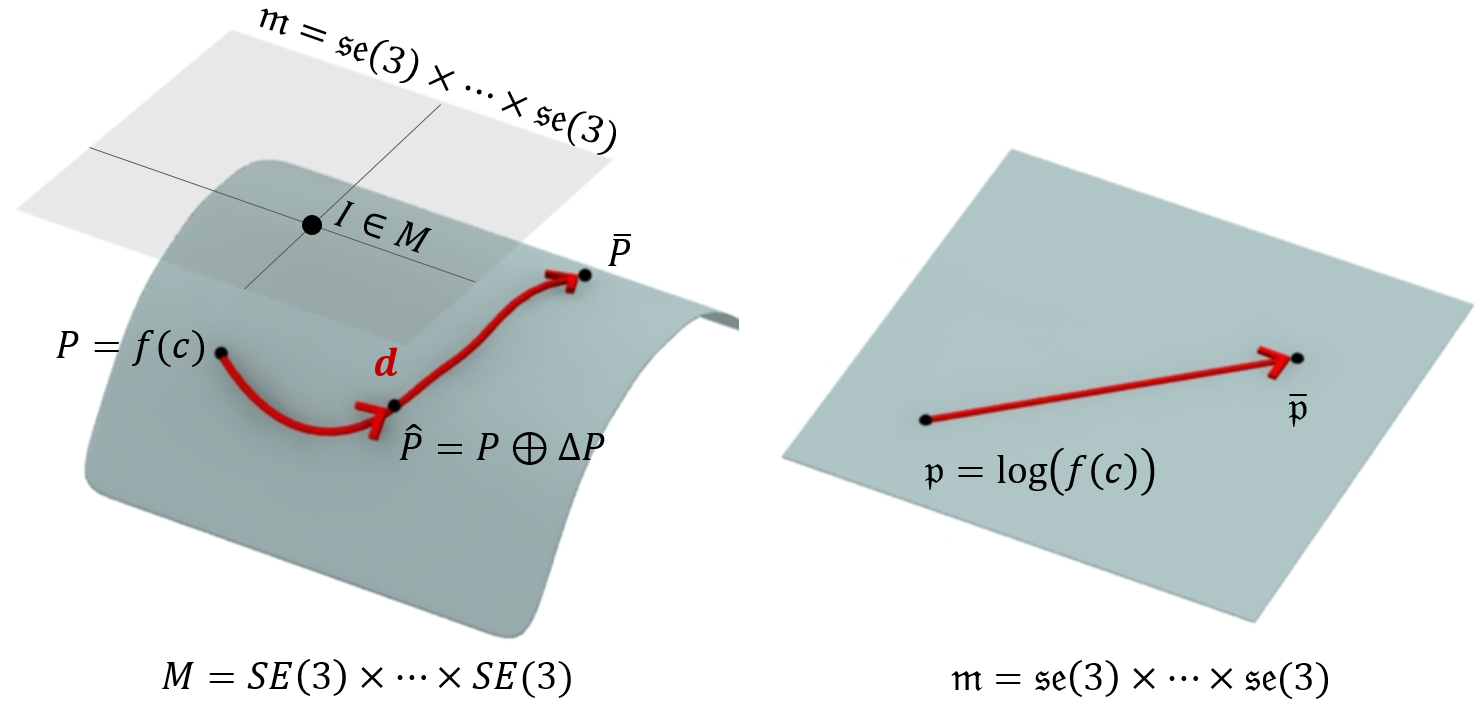
\includegraphics[width=1.0\linewidth]{images/se3}
  \caption{Problem definition of rig space parameter optimization on \SE{} Lie group and its corresponding \se{} Lie algebra.}
  \label{fig:se3}
\end{figure}
To avoid above problems, we opt to perform optimization on manifold.
Figure~\ref{fig:se3} shows a geometrical representation of our rig space optimization. Current pose $\mathbf{p}(i)$ generated by the rig and target pose $\bar{\mathbf{p}}(i)$ can be represented as two different points on a curved manifold Lie group $M = SE(3)\times ... \times SE(3)$.
$d(i)$ denotes the geodesic distance from $\mathbf{p}(i)$ to $\bar{\mathbf{p}}(i)$.
Update of $\mathbf{c}(i)$ by the addition of $\Delta{}\mathbf{c}(i)$ results in update of the pose.
%The new pose $\mathbf{p'}(i)$ and $\mathbf{p}^*(i)$ can be computed as follows:
The new pose $\hat{\mathbf{p}}(i)$ can be computed as follows:

\begin{equation}
	\hat{\mathbf{p}}(i) = \mathbf{p}(i)\oplus\Delta \mathbf{p}(i) = f(\mathbf{c}(i)+\Delta{}\mathbf{c}(i)),
\end{equation}

%\begin{equation}
%	\begin{split}
%	\mathbf{p'}(i) &= \mathbf{p}(i)\oplus\Delta \mathbf{p}(i) = f(\mathbf{c}(i)+\Delta{}\mathbf{c}(i))\\
%	mathbf{p}^*(i) &= \mathbf{p}(i)\oplus d(i) = f(\mathbf{c}(i)+\Delta{}\mathbf{c}^*(i))
%	\end{split}
%\end{equation}

%where operator $\oplus$ is a generalized addition operator on $M$. Thus, our goal is to find the optimal $\Delta{}\mathbf{c}^*(i)$ that minimizes $d(i)$.
where operator $\oplus$ is a generalized addition operator on $M$. Thus, our goal is to find the optimal $\Delta{}\mathbf{c}^*(i)$ that results in the closest point to $\bar{\mathbf{p}}(i)$, which is equivalent to minimize $d(i)$.
However, it is not easy to measure $d(i)$ on a curved manifold $M$.
Therefore, we map the character poses into a Lie algebra $\mathfrak{m} = \mathfrak{se}(3)\times \ldots \times \mathfrak{se}(3)$ that spans the tangent space at the identity element $\mathbf{I}$ of $M$.
This process is performed by the logarithm map(Equation \ref{eq:logmap}) of $SE(3)$, which is known as the \textit{linearization} of the manifold $SE(3)$.
The updated pose using the Lie algebra can be computed as follows:

\begin{equation}
	\hat{\mathfrak{p}}(i) = \mathfrak{p}(i)+\Delta \mathfrak{p}(i) = \mathbf{log}\left(f(\mathbf{c}(i)+\Delta{}\mathbf{c}(i))\right),
\end{equation} 

%\begin{equation}
%	\begin{split}
%		\mathfrak{p}(i)' &= \mathfrak{p}(i)+\Delta \mathfrak{p}(i) = f(\mathbf{c}(i)+\Delta{}\mathbf{c}(i)) \\
%		\mathfrak{p}^*(i) &= \mathfrak{p}(i)+ \mathfrak{d}(i) = f(\mathbf{c}(i) + \Delta{}\mathbf{c}^*(i))\\ 
%	\end{split}
%\end{equation} 
where $\mathfrak{p}(i)$ and $\hat{\mathfrak{p}}(i)$ denotes the Lie algebra vector representation corresponding to a Lie group pose $\mathbf{p}(i)$ and $\hat{\mathbf{p}}(i) $, respectively.
%where $\mathfrak{p}(i)$ denotes the Lie algebra vector representation corresponding to a Lie group pose $\mathbf{p}(i)$, and $\mathfrak{d}(i)$ denotes the distance from $\mathfrak{p}(i)$ to $\mathfrak{p}^*(i)$ on $\mathfrak{m}$.
%Then, we perform the linearized optimization to achieve our rig space motion mapping purposes. 
Since manifold $\mathfrak{m}$ behaves like Euclidean space for small values, we can carry out the linearized optimization on it.

\subsection{Proposed representation}

\begin{figure}[ht]
  \centering
  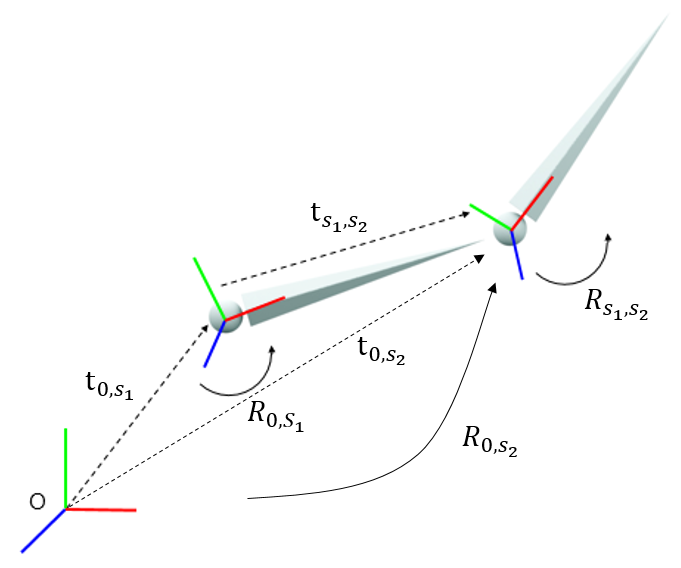
\includegraphics[width=2.5in]{images/rigidBody}
  \caption{Representation of rigid body segment $s_1$ and $s_2$. $R$ is $3\times 3$ rotaiton matrix and $\mathbf{t}\in \mathbb{R}^{3}$ is the vector that represents translation of the segment in the local coordinate systems.}
  \label{fig:rigidbody_example}
\end{figure}

In this section, we introduce a novel skeletal pose representation that couples the hierarchical skeletal structure and the global positions of each skeletal segment. Figure \ref{fig:rigidbody_example} shows a simple example of the hierarchical skeleton structure composed of two skeletal segments $s_0$ and $s_1$. Rigid body transformation of each skeletal segment is a member of Lie group $SE(3)$:
\begin{equation}
	\begin{split}
		A_{0,s_1} & =
		\begin{bmatrix}
			R_{0,s_1} & \mathbf{t}_{0,s_1}\\ 
			0&1
		\end{bmatrix} \in SE(3),\\  
		A_{s_1,s_2} & =
		\begin{bmatrix}
			R_{s_1,s_2} & \mathbf{t}_{s_1,s_2}\\ 
			0&1  
		\end{bmatrix} \in SE(3),\\
	\end{split}
\end{equation}

where $A_{0,s_1}$ is the $SE(3)$ group of the rigid transformation from the global coordinate system to $s_1$, and $A_{s_1,s_2}$ is the $SE(3)$ group of the relative transformation from the local coordinate system $s_1$ to $s_2$. Thus, for the hierarchical skeleton structure of arbitrary rigid skeletal segments $\mathbf{s} = \left \{ s_1, s_2, \dots, s_k\right \}$, the skeletal pose $\mathbf{p}$ can be represented as the direct product of $SE(3)$ Lie group or its corresponding Lie algebra:

\begin{equation}
\begin{split}
	\mathbf{p}_{ s_1, s_2, \ldots, s_k} &= A_{0,s_1} \times \ldots \times A_{s_{k-1},s_k} \times A_{0,s_2} \times \ldots \times A_{0,s_k}\\
	&\in SE(3) \times \ldots \times SE(3),\\
	\mathfrak{p}_{ s_1, s_2, \ldots, s_k} &= \mathrm{vec}_{0, s_1} \times \ldots \times \mathrm{vec}_{s_{k-1},s_k} \times \mathrm{vec}_{0, s_2} \times \ldots \times \mathrm{vec}_{0,s_k}\\
	&\in \mathfrak{se}(3) \times \ldots \times \mathfrak{se}(3),
\end{split}
\end{equation}

where $\mathrm{vec}$ denotes 6 dimensional vector representation of the Lie algebra, and $\mathfrak{p}$ is $6(2k-1)$ dimensions to represent $k$ segments.
Note that we utilize the global transform $A_{0,s}$ of each skeletal segment. Using the hierarchical rigid body transformation($A_{0,s_1} \times A_{s_1,s_2} \times \ldots \times A_{s_{k-1},s_k}$) alone does not provide satisfactory results due to accumulation of the error from the parent body to the child body through hierarchy in terms of global body positions.
With this representation, we could perform accurate and efficient optimization compared to other Euclidean pose representations.
%To remedy this problem, we utilize global positions of each body part.

%\begin{equation}
%	\begin{split}
%		S_{s_1, s_2, ..., s_k} &= p_0\times...\times p_k \times\mathrm{vec}_{0, s_1} \times \ldots \times \mathrm{vec}_{s_{k-1},s_k} \\ 
%		&\in \mathbb{R}^{3}\times ... \times\mathbb{R}^{3} \times \mathfrak{se}(3) \times ... \times \mathfrak{se}(3),
%	\end{split}
%\end{equation}
%
%where $p_s$ is the global position of the rigid skeletal segemnt $s$, and $S$ is our pose represenation vector with $9 \times k$ dimensions to represent $k$ segments. With this representation, we could perform accurate and efficient optimization compared to other Euclidean pose representations.

%\section{previous Method}
%\subsection{Special Euclidean Group SE(3)}
%
%We will briefly introduce special Euclidean group SE(3). Rigid character motion, as like a human body motion, can be represented as an articulated system of rigid segments[V.M.Zatsiorsky. Kinematics of Human Motion]. Mathematically, 3D rigid motions are members of the special Euclidean Group SE(3)[R.M.Murray et al, A Mathematical Introduction to Robotic Manipulation.]. The SE(3) is the set of all 4x4 matrices of the form 
%
%\begin{equation}
%	A(R,\mathbf{t}) =
%		\begin{bmatrix}
%			R & \mathbf{t}\\ 
%			0 & 1
%		\end{bmatrix}
%\end{equation}
%
%where $R \in \mathbb{R}^{3 \times 3}$ is a rotation matrix, $t \in \mathbb{R}^{3}$ is a translation vector. We can combine multiple SE(3) using the direct product x, then the rigid body character pose can be represented as a point on the Lie group SE(3)x...xSE(3), which is a curved manifold(Figure 3).
%The tangent space at the identity of SE(3) is known as the Lie algebra of SE(3), denoted by se(3). The se(3) is 6 dimensional vector space formed by all 4x4 matrices of the form:
%
%\begin{equation}
%	S =
%	\begin{bmatrix}
%		\Omega  & \mathbf{v}\\ 
%		0 & 0
%	\end{bmatrix}
%	=
%	\begin{bmatrix}
%		0 & -\omega_{3} & \omega_{2} & v_{1}\\ 
%		\omega_{3} & 0 & -\omega_{1} & v_{2}\\ 
%		-\omega_{2} & \omega_{1} & 0 & v_{3}\\ 
%		0 & 0 & 0 & 0
%	\end{bmatrix}
%	\in se(3)
%\end{equation}
%
%where $w \in \mathbb{R}^{3}$ and $U$ is a $3\times3$ skew-symmetric matrix. Any element of the matrix can be represented as a vector given by
%\begin{equation}
%	\mathrm{vec}(S)=\left [ \omega_{1},\omega_{2},\omega_{3},v_{1},v_{2},v_{3} \right ]
%\end{equation}
%and the Lie algebra  of combined Lie group $SE(3)\times ...\times SE(3)$ is also represented by direct product $se(3)\times ...\times se(3)$. 
%
%Mapping between Lie group SE(3) and Lie algebra se(3) can be achieved by the exponential map $\mathrm{exp}_{SE(3)}: se(3) \rightarrow SE(3)$ and the logarithm map $\mathrm{log}_{SE(3)} : SE(3)\rightarrow se(3)$ are given by:
%
%\begin{equation}
%	\label{eq:logmap}
%	\mathrm{exp}_{SE(3)}(S) = \mathbf{e}^{S},\\\\
%	\mathrm{log}_{SE(3)}(A) = \mathbf{log}(A)
%\end{equation} 
%where $e$ and $\mathrm{log}$ denote the matrix exponential and logarithm respectively. 
%
%\subsection{Rig optimization on Lie Group}
%Given the input motion $P^*=\left\{\mathbf{p}^*_i|i=1,...,n\right\}$ where $\mathbf{p}^*_i$ is a desired skeletal pose at frame $i$, our problem is to find the optimal sequence of rig space parameters $C=\left\{\mathbf{c}_i|i=1,...,n\right\}$ where $\mathbf{c}_i$ is rig space parameters at frame $i$. %that aims to generate pose equal to $\mathbf{p}^*_i$.
%This task can be formulated as a following least square optimization problem:
%\begin{gather}
%	\min_{C}{\sum_{i=1}^{n}{D(\mathbf{c}_i,\mathbf{p}^*_i)}}, \\%\text{ where}\\
%	\begin{aligned}
%	~D \left( \mathbf{c}_{i},\mathbf{p}^*_{i}\right) &= \left(f\left(\mathbf{c}_{i} \right) - \mathbf{p}_{i}^{*}\right)^T\left(f\left(\mathbf{c}_{i} \right) - \mathbf{p}_{i}^{*}\right)\\
%	&=\left | f(\mathbf{c}_i)-\mathbf{p}_i^* \right |^{2}
%	\end{aligned}\notag
%\end{gather}
%
%%Here, $p_i$, equivalent to $f(\mathbf{c}_i)$, is a pose updated by rig space parameters $\mathbf{c}_i$ and rig function $f(.)$
%where $f(\mathbf{c}_i)$ is a rig function to update skeletal pose at frame $i$ by rig space parameters $\mathbf{c}_i$, 
% $D$ is a distance between the target pose $\mathbf{p}^*_i$ and the updated pose $f(\mathbf{c}_i)$.
%During the optimization, $\mathbf{c}_i$ is updated iteratively by small incremnets:
%\begin{equation}
%	\mathbf{c}_i\leftarrow \mathbf{c}_i+\delta 
%\end{equation}
%where increments $\delta$ are obtained by solving the follwing equation:
%\begin{equation}
%	\left.\begin{matrix}
%	\frac{\partial D(\mathbf{c}_i+\delta) }{\partial\delta }
%	\end{matrix}\right|_{\delta=0} = 0
%\end{equation}
%since a null derivative means a minimum of distance function $D$.
%We iterate above steps until convergence or for a fixed number of iterations. 
%
%%Here, our purpose is find the optimal $C$ that minimizes the error function $D$. Then we would have to store the pose as a vector and measure the distance. 
%%The problem to be solved in optimization requires the distance between two poses. 
%%Here, our optimization work properly on euclidean vector spaces, but naive representation of pose does not form this.
%%The problem to be solved in optimization requires the careful selection of pose representation since it only works properly on euclidean vector spaces.
%Notice our optimization is minimize the error between given target skeletal pose and the rigged character's skeletal pose, thus we would have to represent the poses as a vector and measure the distance. Although there are several possible ways to represent the character pose in Euclidean space, none of them are an ideal solution due to the following reasons:
%\begin{itemize}
%  \item 3D Joint position cannot represent the orientation and rotation of body segment correctly.
%  \item 3D Yaw-Pitch-Roll angles has the singularities causing the "gimbal lock" problem.
%  \item Quaternion is overparameterized, which can cause the optimization method try to optimize free DOF which actually do not exist.
%  \item Elements of transformation matrix has more extra DOF which can cause worse problem. A huge storage requirements is also a drawback.
%\end{itemize}
%
%\begin{figure}[ht]
%  \centering
%  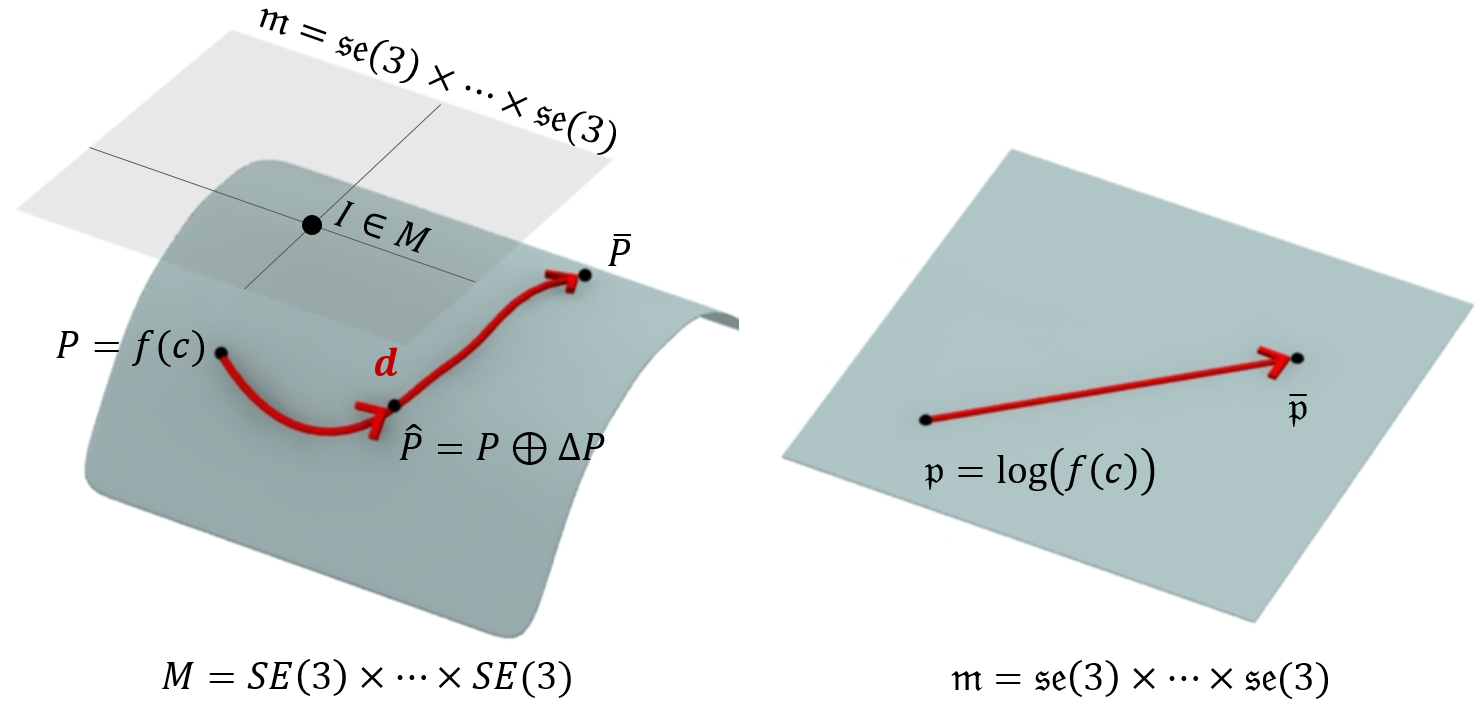
\includegraphics[width=3.0in]{images/se3}
%  \caption{Problem definition of Rig space parameter optimization on SE(3)x..xSE(3) Lie group and its corresponding se(3)x...xse(3) Lie algebra.}
%  \label{fig:manifold_opt}
%\end{figure}
%An elegant solution is optimize on the manifold\cite{blanco2010tutorial}.
%Figure~\ref{fig:manifold_opt} shows the geometrical representation of our rig space optimization. The rig function $f(.)$ updates character pose by changes of rig space parameter $\mathbf{c_{i}}$. The current rig character pose $\mathbf{p}_i$ and target pose $\mathbf{p}_i^*$ can be represented as a point on curved manifold Lie Group $M = SE(3)\times ... \times SE(3)$, respectively. $d_{geo}$ denotes the geodesic path from $\mathbf{p}_i$ to $\mathbf{p}_i^*$. If $\mathbf{c}_i$ is changed by $\delta$, the new pose $\mathbf{p'}_i$ and $\mathbf{p}_i^*$ are represented as follows:
%
%\begin{equation}
%\begin{split}
%\mathbf{p'}_i &= \mathbf{p}_i\bigoplus\Delta \mathbf{p}_i = f(\mathbf{c}_i+\delta) \\
%\mathbf{p}_i^{*} &= \mathbf{p}_i\bigoplus d_{geo} = f(\mathbf{c}_i+\delta ^{*})\\ 
%\end{split}
%\end{equation}
%
%where operator $\bigoplus$ is generalized addition operator on $M$. Thus, our goal is to find an optimal $\delta ^*$ that minimizes the $d_{geo}$.
%However, it is not a trivial task to measure the geodesic distance on the curved manifold such as $M$.
%Therefore, we map the character poses into a Lie algebra $m = se(3)\times ... \times se(3)$, the tangent space at the identity element $\mathbf{I}$ of $M$.
%This process is performed by logarithm map(equation \ref{eq:logmap}) of $SE(3)$, which is called the ''linearization'' of the manifold $SE(3)$\cite{blanco2010tutorial}.
%Thus, our pose measurement on the Lie algebra is represented as follows:
%\begin{equation}
%	\begin{split}
%		\mathfrak{p}_i' &= \mathfrak{p}_i+\Delta \mathfrak{p}_i = f(\mathbf{c}_i+\delta) \\
%		\mathfrak{p}_i^{*} &= \mathfrak{p}_i+ d = f(\mathbf{c}_i + \delta ^{*})\\ 
%	\end{split}
%\end{equation} 
%where $\mathfrak{p}_i$ denotes the Lie algebra vector representation corresponding to a Lie group pose $\mathbf{p}_i$, and $d$ denotes the pose distance on the $m$.
%%Then, we perform the linearized optimization to achieve our rig space motion mapping purposes. 
%Since manifold $m$ behaves like a Euclidean space (for small values), we can carry out the linearized optimization on it.
%
%\subsection{Proposed representation}
%
%\begin{figure}[ht]
%  \centering
%  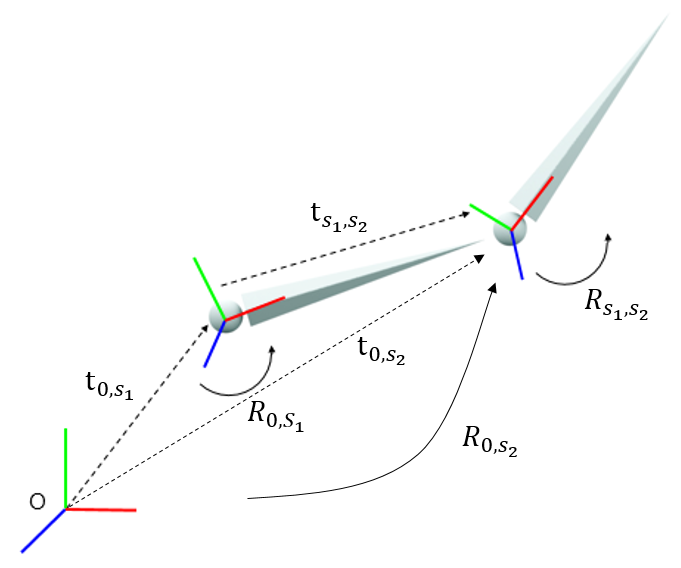
\includegraphics[width=3.0in]{images/rigidBody}
%  \caption{Representation of Rigid body segment $s_1$ and $s_2$. $R$ is $3\times 3$ rotaiton matrix and $t\in \mathbb{R}^{3}$ vector that represents transformations of the segment in the local coordinate systems. $p\in \mathbb{R}^{3}$ is global position of the body segment.}
%  \label{fig:2}
%\end{figure}
%
%In this section, we introduce a novel skeletal pose representation which couples hierarchical skeletal structure and global positions of each skeletal segment. Figure 2 shows the simple example of hierarchical skeleton structure is composed of two rigid body segments. Rigid body transformation of each segment is member of Lie group SE(3), 
%
%\begin{equation}
%	\begin{split}
%		A_{0,s_1} =
%		\begin{bmatrix}
%			R_{0,s_1} & \mathbf{t}_{0,s_1}\\ 
%			0&1
%		\end{bmatrix} \in SE(3)\\  
%		A_{s_1,s_2} =
%		\begin{bmatrix}
%			R_{s_1,s_2} & \mathbf{t}_{s_1,s_2}\\ 
%			0&1  
%		\end{bmatrix} \in SE(3)\\
%	\end{split}
%\end{equation}
%
%
%where $A_{(0,s_1)}$ is SE(3) group of the rigid transformation from the global coordinate system to the $s_1$, and $A_{(s_1,s_2)}$ is the SE(3) group of the relative transformation from the local coordinate system $s_1$ to $s_2$. Thus, for the hierarchical skeleton structure of arbitary rigid body segments $\left \{ s_1, s_2, …, s_k\right \}$, the pose $P$ is represented as direct product of SE(3) Lie Group and its corresponding Lie algebra:
%
%\begin{equation}
%\begin{split}
%	P_{ s_1, s_2, ..., s_k} = A_{0,s_1} \times...\times A_{s_{k-1},s_k} \in SE(3) \times ... \times SE(3) \\
%	\mathfrak{p}_{ s_1, s_2, ..., s_k} = \mathrm{vec}_{0, s_1} \times... \times \mathrm{vec}_{s_{k-1},s_k} \in se(3) \times ... \times se(3)
%\end{split}
%\end{equation}
%
%where $\mathrm{vec}$ denotes 6 dimensional vector representation of the Lie algebra. However, during the our optimization process we notices that only using the hierarchical rigid body transformation is not enough because the error of parent body segment is accumulated to the child segments. To remedy such error, we also used the global positions $p\in\mathbb{R}^{3}$of each body part. Thus, our proposed skeletal pose representation is:
%
%\begin{equation}
%	\begin{split}
%		S_{s_1, s_2, ..., s_k} = p_0\times...\times p_k \times\mathrm{vec}_{0, s_1} \times... \times \mathrm{vec}_{s_{k-1},s_k} \\ 
%		\in \mathbb{R}^{3}\times ... \mathbb{R}^{3} \times se(3) \times ... \times se(3)
%	\end{split}
%\end{equation}
%
%where $p_n$ is global position of the rigid body segemnt, S is our proposed pose represenation vector which is dimension 9xk to represent $k$ segments. With this representation, we could perform more correct and efficient optimization than other euclidean pose representations. 



%%%%%%%%%%%%%%%%%%%%%%%%%%%%%%%%%%%%%%%%%%%%%%%%%%%%%%%%%%%%%%%%%%%%%%%%%%%%
%%old



%\begin{figure}[ht]
%  \centering
%  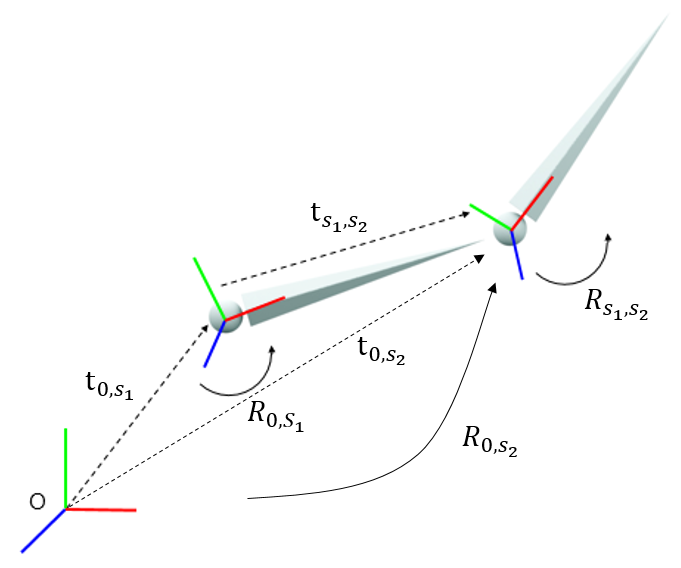
\includegraphics[width=3.0in]{images/rigidBody}
%  \caption{Representation of Rigid body segment $e_n$ and $e_m$.}
%  \label{fig:2}
%\end{figure}



%Figure 2 shows the simple example of hierarchical skeleton structure composed of rigid body segment. $B_{n,m} = (e_n, e_m)$ is skeleton structure composed of rigid body segment $e_n$ and $e_m$, and each of $(e_{ns}, e_{ne}),(e_{ms}, e_{me}) \in \mathbb{R}^3$ is starting and end point of $e_n$ and $e_m$. $I_n$ and $I_m$ are scalar values that represents the length of each segment. The local coordinate system of $e_n$ can be obtained by rotating and translating the global coordinate system, with its origin at the $e_{ns}$, X-axis aligned with the $e_{ne}$ direction. At time step t, the starting and end point $e^{0}_{ns(t)},  e^{0}_{ne(t)} \in \mathbb{R}^3$ can be represented as following equation:


%\begin{equation}
%\begin{bmatrix}
%e^{0}_{ns}(t) & e^{0}_{ne}(t)\\ 
%1 & 1
%\end{bmatrix}
%=
%\begin{bmatrix}
%R_{0,n}(t) & \mathbf{t}_{0,n}(t)\\ 
%0 & 1 
%\end{bmatrix}
%\begin{bmatrix}
%0 & l_{n}\\ 
%0 & 0\\ 
%0 & 0\\ 
%1 & 1
%\end{bmatrix}
%\end{equation}

%where $R_{0,n(t)}$ and $t_{0,n(t)}$ are rotation and translation matrix from global coordinate to local coordinate.

%Also, $e_m$ which is the child body part of $e_n$ can be represented in local coordinate system :
%\begin{equation}
%\begin{bmatrix}
%e^{n}_{ms}(t) & e^{n}_{me}(t)\\ 
%1 & 1
%\end{bmatrix}
%=
%\begin{bmatrix}
%R_{n,m}(t) & \mathbf{t}_{n,m}(t)\\ 
%0 & 1 
%\end{bmatrix}
%\begin{bmatrix}
%0 & l_{m}\\ 
%0 & 0\\ 
%0 & 0\\ 
%1 & 1
%\end{bmatrix}
%\end{equation}
%Since the length of each body segment $l_n$ and $l_m$ is unchanged, the transformation matrix in equation (5) and (6) can be represented as SE(3) Lie Group:

%\begin{equation}
%\begin{split}
%	A_{0,n}(t) = \begin{bmatrix}
%				R_{0,n}(t) & \mathbf{t}_{0,n}(t)\\ 
%				0 & 1
%				\end{bmatrix}\\
%	A_{0,m}(t) = \begin{bmatrix}
%				R_{0,m}(t) & \mathbf{t}_{0,m}(t)\\ 
%				0 &1  
%				\end{bmatrix}\\
%	A_{n,m}(t) = \begin{bmatrix}
%				R_{n,m}(t) & \mathbf{t}_{n,m}(t)\\ 
%				0 &1  
%				\end{bmatrix}
%\end{split}
%\end{equation}

%
%Although the rigid body transformation of $e_n$ and $e_m$ can be represented by $\left \{ A_{(0,n)}, A_{(n,m)} \right \}$, it is not suitable in optimization process since the hierarchical rigid body system accumulate the error of the parent body to the child body. To remedy such error, we also used each body segment's transformation matrix from the global frame. Thus, for the hierarchical rigid body structure of rigid skeleton segment $\left \{ e_1, e_2, …, e_k\right \}$, the pose $P$ at time t is represented as $2k-1$ dimension of SE(3) Lie Group :

%\begin{equation}
%\begin{split}
%	P_{ e_{1},e_{2},...,e_{k}}(t) = A_{0,1}(t) \times...\times A_{0,k}(t) \times{} \\
%	A_{1,2}(t) \times ... \times A_{e_{k-1},e_{k}}(t) 
%\end{split}
%\end{equation}

%where $\times$ is direct product.

%However, it is difficult to minimize the distance on Curved manifold SE(3)x..xSE(3) Lie Group. (Figure 3)
%Therefore, we mapped the SE(3)x...xSE(3) Lie Group P into corresponding Lie algebra using logarithm map :

%\begin{equation}
%\begin{split}
%\mathfrak{p}_{e_{1},e_{2},...,e_{k}}(t) = [\mathrm{vec}(\mathbf{log}(A_{0,1}(t)), ..., \mathrm{vec}(\mathbf{log}(A_{0,k}(t)),\\
%\mathrm{vec}(\mathbf{log}(A_{1,2}(t)), ..., \mathrm{vec}(\mathbf{log}(A_{k-1, k}(t))] \\
%\in se(3) \times ... \times se(3)
%\end{split}
%\end{equation}

%where $\mathfrak{p}(t)$ is a vector representation of Lie algebra which is dimension 6x2x(k-1) at any time instance t. 
%This mapping method is called linearization of Lie Group Manifold\cite{blanco2010tutorial}. Using this method, we can linearly optimize(minimize) the distance of skeletal pose in Lie algebra space\cite{blanco2010tutorial}.

%Figure 3 shows geometrical representation of our rig space optimization. The $f$ is rig function, and $C$ is rig space parameter. The current rigid body character pose $f(c)$ is the point P on curved manifold Lie Group $SE(3)\times ... \times SE(3)$. The $P^*$ is the target pose given by input, and $\Delta{P_{geo}}$ is the geodesic path from current pose $P$ to target pose $P^*$. If the rig space parameter $C$ is changed by $\Delta{C}$, the new pose $P’$ and the target pose $P^*$ is represented as follows:
%\begin{equation}
%P' = P+\Delta P = f(C+\Delta C) \\
%\end{equation}
%\begin{equation}
%P^{*} = P+\Delta P_{geo} = f(C+\Delta C^{*}) \\
%\end{equation}
%\begin{equation}
%d_{geo} = \Gamma (\Delta P_{geo})
%\end{equation}
%where $\Gamma(x)$ is geodesic distance function, $d_{geo}$ is Lie Group geodesic distance of $\Delta{P_{geo}}$.
%Our goal is find the optimal difference of Rig space parameter $\Delta C^*$ that minimize the $\Delta P_{geo}$.
%Although it is not trivial to represent the geodesic distance function $\Gamma(x)$ in explicit form, we can replace it with the distance in Lie algebra space through the linearization process (equation 9) and successfully optimize the rig space parameter $\Delta C^*$.
